\chapter{Integrals of motion}
\thispagestyle{chapterBeginStyle}

\paragraph{}The problem of our interest is the systematic classification of all local and quasilocal integrals of
motion (LIOMs and QLIOMs) supported on \( m \in \NN \) sites in a model given by 1-D tight-binding Hamiltonian \(H\). 
To this end, we employ the algorithm first proposed in~\textcite{Mierzejewski2015a}. It allows us to classify integrals
of motions for a given system size \(L\). After doing so for accessible values of \(L\), we then carry out finite size scaling
to obtain information about the thermodynamic limit \(L \to \infty \). 

In our description and notation used, we will  follow
the works of~\textcite{Mierzejewski2015a,Mierzejewski2015Approx,Mierzejewski2018}.
The aim of this thesis is to provide a pedagogical introduction to the topic,
so all derivations are presented in full detail, together with a simple proof of correctness for the algorithm.

%%%%%%%%%%%%%%%%%%%%%%%%%%%%%%%%%%%%%%%%%%%%%%%%%%%%%%%%%%%%%%%%%%%%%%%%%%%%%%%%%%%%%%%%%%%%%%%%%%%%%%%%%%%%%%%%%%%%%%%%%%%%%%%%
\section{Preliminaries}

\paragraph{Space of observables}Consider the vector space \(\mathcal{V}_L\) of traceless and translationally invariant
observables, acting on a Hilbert space of dimension \(2^L\). We can define an inner product on this space:
\begin{equation}
  \hs{A}{B} = \frac{1}{2^L}\tr(A^{\dagger}B) = \frac{1}{2^L} \sum_{mn} A_{nm}B_{nm}^{\ast}
\end{equation}
i.e.\;the Hilbert-Schmidt product, where \(A_{nm} = \matrixel{n}{A}{m}\) and \(H\ket{n} = E_n \ket{n}\). Moreover,
we define the Hilbert-Schmidt norm of an operator to be \(\norm{A} = \sqrt{\hs{A}{A}}\).
These definitions are correct, as we work only with finite dimensional Hilbert spaces and taking the trace is an
linear operation. We require the operators to be traceless, because they have zero overlap with the identity, \(\left(A|\Id\right)=\frac{1}{2^L}\tr(A) = 0\).
Now we consider a subspace \(\mathcal{V}_L^m\) of \(m\)-local operators and a direct sum
\(\mathcal{V}_L^M = \bigoplus_{m = 1}^M \mathcal{V}_L^m\) being a subspace of operators supported on up to \(M\) sites.
We also define a basis of \(\mathcal{V}_L^M\) consisting of operators \(O_s\in \mathcal{V}_L^M\)
satisfying the following properties:
\begin{align}
   & \hs{O_s}{O_{t}} = \delta_{s,t} \tag{\text{orthonormality}}                                    \nonumber{}\\
   & \big(\forall A \in \mathcal{V}_L^M\big) \big(A = \sum_s \hs{O_s}{A} O_s\big) \tag{\text{completeness}}   \nonumber{}\\
   & \big(\forall A \in \mathcal{V}_L \big) \big( A = A^M + A^{\perp} = \sum_s \hs{O_s}{A} O_s + A^{\perp}\big) ,
  \text{ such that } \big(\forall s\big) \big( \hs{O_s}{A^{\perp}} = 0\big)\label{eq:basis}
\end{align}


\paragraph{Locality} We begin with a definition of integral of motion in quantum mechanics.
\begin{definition}
  Let \(H\) be a Hamiltonian operator. Then, any observable \(O\) fulfilling the equation:
  \[
    \comm{H}{O} = 0
  \]
  is an \textbf{integral of motion}.\label{def:iom}
\end{definition}
It is easy to see, that there are many such observables. Let us consider the following
\begin{example}
  Take \(H\) to be any Hamiltonian operator. By spectral theorem, it can be written is diagonal form:
  \begin{equation*}
    H = \sum_n E_n \ketbra{n}{n}
  \end{equation*}
  Then a set of projection operators \(P_n = \ketbra{n}{n}\) is a family of IOMs.
  Eigenstates of a Hamiltonian are in general very nonlocal.\label{ex: projectors}
\end{example}
However, as it will become evident in Section~\ref{sec:spectral function} on spectral function, nonlocal operators are not important in the
thermodynamic limit and we are only interested in the so called local (or quasilocal) integrals of motion.
A working intuition behind local operators is perhaps best seen in Figure~\ref{fig:1D chain}. They can be thought of as
being different from identity only on \(m\) consecutive sites. XXZ Hamiltonian defined by equation~\eqref{eq:HXXZ} is an
example of 2-local operator. On the other hand, quasilocal operator can be represented as a convergent sum of operators
with increasing support.
\begin{figure}[!htbp]
  \centering
  \hspace*{-0.5cm}
  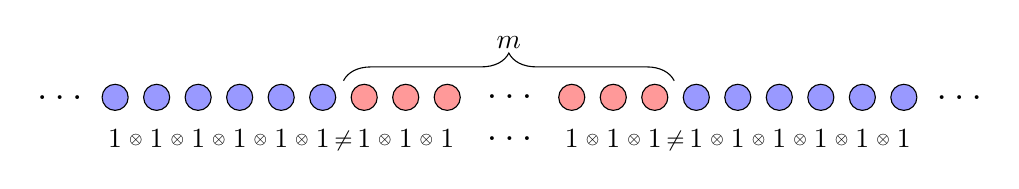
\begin{tikzpicture}[node distance = 15pt, auto]
    \tikzstyle{line} = [draw, -latex',thick]
    \tikzstyle{site1}=[circle, draw, fill=blue!40]
    \tikzstyle{site2}=[circle, draw, fill=red!40]
    % Place nodes

    \node [site1] (site-1) at (-8, 0) {};
    \foreach \x / \name in {1/2,2/3,3/4,4/5,5/6}
    \node [site1, right of=site-\x] (site-\name) {};

    \node [site2, right of =site-6] (site-7){};
    \foreach \x / \name in {7/8,8/9}
    \node [site2, right of=site-\x] (site-\name) {};

    \node [site2, right of=site-9, node distance=45pt] (site-10){};
    \foreach \x / \name in {10/11,11/12}
    \node [site2, right of=site-\x] (site-\name) {};

    \node[site1, right of=site-12] (site-13){};
    \foreach \x / \name in {13/14,14/15,15/16,16/17,17/18}
    \node [site1, right of=site-\x] (site-\name) {};

    \node [left of=site-1, node distance=20pt] {\Large $ \ldots $};
    \node [right of=site-18, node distance=20pt] {\Large $ \ldots $};


    \foreach \x in {1,...,18}
    \node [black, below of=site-\x](op-\x) {\(\mathbb{1}\)};

    \foreach \x / \y in {1/2,2/3,3/4,4/5,5/6,7/8,8/9,10/11,11/12,13/14,14/15,15/16,16/17,17/18}
    \path[draw=none] (op-\x) -- (op-\y) node [black,midway,yshift=-6pt] {\tiny$\otimes$};

    \path[draw=none] (op-6) -- (op-7) node [black,midway,yshift=-8pt] {\footnotesize$\neq$};
    \path[draw=none] (op-12) -- (op-13) node [black,midway,yshift=-8pt] {\footnotesize$\neq$};
    % \foreach \x in {-1.5,-1.0,-0.5,0.5,1.0,1.5}
    % \node [site2] (site-\x) at (\x, 0) {};

    \draw [decorate,decoration={brace,amplitude=10pt},yshift=6pt]
    (-5.1,0) -- (-0.9,0) node [black,midway,yshift=8pt] {$m$};

    \path [draw=none] (site-9) -- (site-10) node [black,midway,yshift=-4pt] {\Large$\ldots$};
    \path [draw=none] (op-9) -- (op-10) node [black,midway,yshift=-4pt] {\Large$\ldots$};
  \end{tikzpicture}
  \caption{Illustration of an operator supported on \(m\) sites.}\label{fig:1D chain}
\end{figure}
In Section~\ref{sec:algorithm}, a precise definition of locality and quasilocality will be stated.

\paragraph{Noncommutativity}In the case of XXZ model (also in general XYZ model) the Hamiltonian preserves the total \(z\)-component of spin,
or in other words, it commutes with the total spin operator of the form:
\begin{equation*}
  \Sz_{tot} = \sum_{i = 1}^{L} \Sz_i
\end{equation*}
This fact allows us to decompose the full Hilbert space into parts consisting of states with the same total \(z\)-component
of spin. In more mathematical terms, we have the following:
\begin{equation*}
  \mathcal{H} = \bigoplus_{i = 0}^{L} \mathcal{H}_i \text{, where } \big(\forall \ket{\psi} \in \mathcal{H}_i \big) \big(\Sz_{tot} \ket{\psi} = \frac{1}{2}(i-L) \ket{\psi} \big)
\end{equation*}
i.e.\;the full Hilbert space with \(\dim{\mathcal{H}} = 2^L\) can be decomposed into the direct sum of its proper subspaces
\(\mathcal{H}_i\) such that \(\dim{\mathcal{H}_i} = \binom{L}{i}\) and all states in a given subspace correspond to the same
eigenvalue of \(\Sz_{tot}\) operator. The index \(i\) denotes the number of sites with spin up.
Now we are ready for
\begin{definition}
  Let \(O\) be an integral of motion. If \(O\) preserves total \(z\)-component of spin, i.e.
  \(\comm{\Sz_{tot}}{O} = 0\), then it is called a \textbf{commuting integral of motion}.
  Otherwise, it is called a \textbf{noncommuting integral of motion}.\label{def:noncomm def}
\end{definition}
For the algorithm described in Section~\ref{sec:algorithm}, we need to construct matrices of
observables and express them in the Hamiltonian eigenbasis. If the operator in question is a
commuting IOM, we can restrict ourselves to the fixed spin subspace and thus greatly reduce
computational complexity, allowing us to investigate larger systems. Such operators, for example
spin energy current, have already been studied~\autocite{Mierzejewski2015Approx}. Therefore,
the main focus of this work is the investigation of existence and properties of much less known
noncommuting IOMs. This forces us to remain in full Hilbert space and restricts system sizes
that we are able to check.

%%%%%%%%%%%%%%%%%%%%%%%%%%%%%%%%%%%%%%%%%%%%%%%%%%%%%%%%%%%%%%%%%%%%%%%%%%%%%%%%%%%%%%%%%%%%%%%%%%%%%%%%%%%%%%%%%%%%%%%%%%%%%%%%

\section{(Q)LIOMs finding algorithm\label{sec:algorithm}}
We now introduce a finite time averaging of an operator \(A\in \mathcal{V}_L^M\), employing the Heisenberg picture~\autocite{Mierzejewski2015Approx}:
\begin{align}
  \bar{A}^{\tau} = & \frac{1}{\tau} \int_0^{\tau} \mathrm{d}t\, A_{H}(t) = \frac{1}{\tau} \int_0^{\tau} \mathrm{d}t\, e^{i H t}A e^{-i H t}
  =\sum_{m,n} \frac{1}{\tau} \int_0^{\tau} \mathrm{d}t\, e^{i E_m t}\ket{m} \matrixel{m}{A}{n}\bra{n}  e^{-i E_n t} = \nonumber{}           \\
  =                & \sum_{m,n} A_{mn}\ketbra{m}{n} \frac{1}{\tau} \int_0^{\tau} \mathrm{d}t \, e^{i(E_m-E_n)t} =
  \sum_{m,n} A_{mn}\ketbra{m}{n} \frac{1}{\tau} \frac{1}{i\left(E_m-E_n\right)}\left(e^{i\left(E_m-E_n\right)\tau}-1\right) \nonumber       \\
  =                & \sum_{m,n} A_{mn}\ketbra{m}{n}
  e^{i\left(E_m-E_n\right)\tau/2}\times \frac{\sin{\left(\left(E_m-E_n\right)\tau\right)}}{\tau\left(E_m-E_n\right)}
  \label{eq:time_avg}
\end{align}
What this procedure does is essentially a cut off \textcolor{blue}{figure illustrating the cut off} of for matrix elements determined by the value of \(E_m-E_n\) in relation
to the averaging time \(\tau{}\). However, this expression is quite complicated and therefore we replace it with a simplified time
averaging (henceforth time averaging):
\begin{definition}
  \begin{equation}
    \bar{A}^{\tau} \equiv \sum_{m,n} \theta\left(\frac{1}{\tau} - \abs{E_m-E_n}\right) A_{mn} \ketbra{m}{n}
    = \sum_{m,n} \theta_{mn}^{\tau} A_{mn} \ketbra{m}{n}
  \end{equation}
  \label{def:simple time avg}
  where \(\theta{}\) is the Heaviside step function, is the time averaged version of operator \(A\).
\end{definition}
Going to the infinite time limit we obtain the time averaging
from~\textcite{Mierzejewski2015a}:
\begin{equation}
  \bar{A} = \lim_{\tau \to \infty} \bar{A}^{\tau} = \sum_{ \substack{m,n\\E_m=E_n} } A_{mn} \ketbra{m}{n}
  \label{eq:inf time avg}
\end{equation}

Observing that \({\left(\theta_{mn}^{\tau}\right)}^2 = \theta_{mn}^{\tau}\) and \({\left(\bar{A}^{\tau}\right)}_{mn} =
\theta_{mn}^{\tau} A_{mn}\) we can easily show some crucial properties of the time averaging:
\begin{proposition}
  For any \(A,B \in \mathcal{V}_L\)
  \begin{equation*}
    \hs{\bar{A}^{\tau}}{\bar{B}^{\tau}} = \hs{A}{\bar{B}^{\tau}} = \hs{\bar{A}^{\tau}}{B}
  \end{equation*}
  and
  \begin{equation*}
    \overline{\left(\bar{A}^{\tau}\right)}^{\tau} = \left(\bar{A}^{\tau}\right)
  \end{equation*}
  \label{prop:projection}
\end{proposition}

\begin{proof}
  \begin{align*}
    \hs{\bar{A}^{\tau}}{\bar{B}^{\tau}}  & = \frac{1}{2^L} \sum_{mn} {\left(\bar{A}^{\tau}\right)}_{mn}
    {\left(\bar{B}^{\tau}\right)}_{mn}^{\ast} = \frac{1}{2^L} \sum_{mn} {\left(\theta_{mn}^{\tau}\right)}^2 A_{mn} B_{mn}^{\ast} \nonumber{}               \\
    & = \frac{1}{2^L} \sum_{mn} \left(\theta_{mn}^{\tau}\right) A_{mn} B_{mn}^{\ast} =
    \hs{A}{\bar{B}^{\tau}} = \hs{\bar{A}^{\tau}}{B}                                                                                                        \\
    \overline{\left(\bar{A}^{\tau}\right)}^{\tau} & = {\left(\theta_{mn}^{\tau}\right)}^2 A_{mn} = \theta_{mn}^{\tau} A_{mn} = \left(\bar{A}^{\tau}\right)
  \end{align*}
  
\end{proof}

These two facts reveal an interesting interpretation of the time averaging, namely that it can be
thought of as an orthogonal projection in vector space \(\mathcal{V}_L\). The involutive character of this operation explains,
why we can consider \(\bar{A}^{\tau}\) time independent in the time window \(\left(0,\tau\right)\).

Let us now calculate the commutator of time-averaged operator with the Hamiltonian:
\begin{align}
  \comm{H}{\bar{A}^{\tau}} & = \sum_n \sum_{k,p} E_n \theta_{kp}^{\tau} A_{kp} \comm{ \ketbra{n}{n}}{ \ketbra{k}{p}} \nonumber         \\
                           & = \sum_{k,p} \left(E_k-E_p\right) \theta_{kp}^{\tau} A_{kp} \ketbra{k}{p} \xrightarrow{\tau \to \infty} 0
\end{align}
The last limit follows directly from equation~\eqref{eq:inf time avg}. We can see that the infinite time averaging procedure
creates an integral of motion, i.e. \(\comm{H}{\bar{A}} = 0\). Nonetheless, it is not enough to just time average a
local operator in order to get a local integral of motion, because in general \(A\in \mathcal{V}_L^M  \nRightarrow \bar{A} 
\in \mathcal{V}_L^M\), that is the truncation of matrix elements modifies the support of an operator.
One possible approach to checking its locality would be to
express this operator in the basis defined in~\eqref{eq:basis}. If for some \(M\) we have \(\bar{A}\in \mathcal{V}_L^M\),
then it is local. Second possibility is that it can be written as a convergent series of operators from \(\mathcal{V}_L^m\) with
increasing \(m\) --- then it is quasilocal. Otherwise it is a generic nonlocal quantity. But can we do better than this
direct approach?

To answer this question, we fix \(0\leq M \leq L/2\) and construct a basis \(\{O_s\}\) of \(\mathcal{V}_L^M\). How to actually perform such construction
will be shown in Section~\ref{sec:example}. Next, we find time averages of all basis operators and build a matrix
\begin{equation}
  K_{st}^{\tau} = \hs{\bar{O_s}^{\tau}}{\bar{O_t}^{\tau}}
\end{equation}
This matrix is Hermitian by design. However, we assume that it is real and symmetric, 
as usually considered operators are of the form \(O+O^{\dagger}\) or \(i\left(O-O^{\dagger}\right)\).
Therefore, the spectral theorem guarantees existence of an unitary matrix \(U\) that
diagonalizes it. In other words, \(D = UK^{\tau}U^{\dagger}\) is diagonal and we have the following relations:
\begin{align}
  &\sum_{s, t} U_{n s} K_{s t}^{\tau} U_{t m}^{T}=\delta_{nm} \lambda_{n} \in \RR,\;\;\; \lambda_n \text{ --- eigenvalue of }K^{\tau} \nonumber \\
  &UU^{\dagger} = U^{\dagger}U = \mathbb{1} \implies \sum_{s} U_{ns}U_{sm}^{T} = \delta_{mn}\nonumber\\
  & U K = D U \implies \sum_s U_{ns} K_{st}^{\tau} = \sum_s  \delta_{ns} \lambda_s U_{st} = \lambda_n U_{nt}\label{eq:properties}
\end{align} 
With the help of the \(U\) matrix (eigenvectors of \(K^{\tau}\)) we can define a new set of rotated operators that
are time-independent in the window \(\left(0,\tau\right)\):
\begin{equation}
  Q_n = \sum_s U_{ns}\bar{O}_{s}^{\tau}\label{eq:new operators}
\end{equation} 

\begin{proposition}
Operators \(Q_n\) are orthogonal, i.e. \(\hs{Q_n}{Q_m} \propto \delta_{nm}\)
\label{prop:orthogonality}
\end{proposition}
\begin{proof}
  Let \(Q_n,Q_m\) be two operators defined as in~\eqref{eq:new operators}.
  Their orthogonality can be shown by direct calculation:
  \begin{align*}
    \hs{Q_n}{Q_m} &= \sum_{s,t} U_{ns} {\hs{\bar{O_s}^{\tau}}{\bar{O_t}^{\tau}}} U_{tm}^{T} 
    = \sum_{t} \left(\sum_{s}U_{ns} K_{st}^{\tau}\right)  U_{tm}^{T} \\ 
    &\triangleq \lambda_n \sum_t U_{nt} U_{tm}^{T} \triangleq \lambda_n \delta_{mn}
  \end{align*}
\end{proof}
The last two equalities, marked with \(\triangleq \), follow from properties~\eqref{eq:properties}. We can learn something more
about the eigenvalues of \(K^{\tau}\) matrix from a simple corollary to Proposition~\ref{prop:orthogonality}.
\begin{corollary}
  \(K^{\tau}\) is a positive semi-definite matrix.\label{corr:psd}
\end{corollary}
\begin{proof}
Let \(Q_n\) be defined as in~\eqref{eq:new operators}. Then, from the defining properties of inner product we have that
\(\hs{Q_n}{Q_n} \geq 0\). However, we also have that \(\hs{Q_n}{Q_n} = \lambda_n\). Combining these two equations, we get
that \(\left(\forall n\right) \left(\lambda_n \geq 0\right)\). Therefore \(K^{\tau}\) is a positive semi-definite matrix.
\end{proof}
This corollary provides us with a lower bound on spectrum of matrix \(K^{\tau}\). 

Let us now examine the support of \(Q_n\). By~\eqref{eq:basis} and making use of~Proposition~\ref{prop:projection}
and properties~\eqref{eq:properties}, we can decompose into \(M\)-local part and nonlocal part:
\begin{align}
  Q_n &=  \sum_s \hs{O_s}{Q_n}O_s + Q_s^{\perp} = \sum_{s,t} U_{n t}\hs{O_{s}}{\bar{O}_{t}^{\tau}}
  O_{s}+Q_{n}^{\perp} \nonumber \\
  &= \sum_{s,t} U_{n t}\hs{\bar{O}_{s}^{\tau}}{\bar{O}_{t}^{\tau}} O_{s}+Q_{n}^{\perp}
  = \sum_{s,t} U_{n t}K_{ts} O_{s}+Q_{n}^{\perp} \nonumber \\
  &= \sum_s  \left( \sum_t U_{n t}K_{ts}^{\tau}\right) O_{s}+Q_{n}^{\perp} = \sum_{s} 
  \lambda_{n} U_{n s} O_{s}+Q_{n}^{\perp} = Q_{n}^{M}+Q_{n}^{\perp}
  \label{eq:decomposition}
\end{align}
Now we are ready to derive central result, stating why this actually algorithm works. Combining the fact that 
\(\hs{Q_n}{Q_n} = \lambda_n \)(see proof of Proposition~\ref{prop:orthogonality}) with~\eqref{eq:decomposition} we obtain:
\begin{align}
  \lambda_n &= \hs{Q_n}{Q_n} = \hs{Q_n^M + Q_n^{\perp}}{Q_n^M + Q_n^{\perp}} = \hs{Q_n^M}{Q_n^M} +
   \hs{Q_n^{\perp}}{Q_n^{\perp}} + \underbrace{2 \hs{Q_n^M}{Q_n^{\perp}}}_{=0 \text{ (cf.~\eqref{eq:basis})}} \nonumber \\
   &= \hs{\sum_s \lambda_n U_{ns} O_s}{\sum_t \lambda_n U_{nt} O_t} + \norm{Q_n^{\perp}}^2 =
  \lambda_n^2 \sum_{s,t} U_{ns} \hs{O_s}{O_t} U_{tn}^{T} + \norm{Q_n^{\perp}}^2  \nonumber \\
  &=\lambda_n^2 + \norm{Q_n^{\perp}}^2
\end{align}
Rearranging the above equality we get that \(\lambda_n - \lambda_n^2 = \norm{Q_n^{\perp}}^2 \geq 0\), which together with
Corollary~\ref{corr:psd} gives \(\lambda_n \in \left[0,1\right]\). 


From now on, we will focus on the case \(\tau \to \infty \), as it guarantees that \(\bar{O_s}\)'s and hence \(Q_n\)'s
commute with the Hamiltonian. 
Consequently, we finally arrive at a classification scheme for the support of \(Q_n\)'s.
\begin{definition}
  An integral of motion \(Q_n\) is called:
  \begin{itemize}
    \item local: \(\lambda_n = 1 \implies \norm{Q_n^{\perp}} = 0 \implies Q_n \in \mathcal{V}^M_L\)
    \item quasilocal: \(\lambda_n \in \left(0,1\right) \implies \norm{Q_n^{\perp}} > 0 \implies Q_n \in \mathcal{V}_L \)
    \item generic: \(\lambda_n = 0 \implies \norm{Q_n} = 0\)
  \end{itemize}
\end{definition}
The procedure outlined above works for a fixed system size \(L\).
In principle, to asses the character of an integral of motion, we need to examine how \(\lambda_n\) behaves in the thermodynamic limit.
To achieve this, we execute this algorithm for a few accessible values of \(L\) and then proceed with finite size scaling.
However, in this thesis we will examine both the \(L\to \infty \) case and \(L = 14\)
case, that is largest system size for exact diagonalization that we were able to attain.


\paragraph{Proof of corectness}

\textcolor{blue}{here the proof that best IOM from the algorithm is the best possible IOM}
We will end this section with a short summary on support of \(Q_n\):
\begin{align}
  & Q_n = Q_n^M + Q_n^{\perp}\nonumber\\
  & \norm{Q_n}^2 = \lambda_n \nonumber\\
  & \norm{Q_n^M}^2 = \lambda_n^2 \nonumber\\
  & \norm{Q_n^{\perp}}^2 = \lambda_n - \lambda_n^2
  \label{eq:summary of support}
\end{align}
%%%%%%%%%%%%%%%%%%%%%%%%%%%%%%%%%%%%%%%%%%%%%%%%%%%%%%%%%%%%%%%%%%%%%%%%%%%%%%%%%%%%%%%%%%%%%%%%%%%%%%%%%%%%%%%%%%%%%%%%%%%%%%%

\section{Spectral functions and Mazur bound\label{sec:spectral function}}

\paragraph{}One may ask a question, why are local (and quasilocal) IOMs actually important. To answer this
question in a convincing manner we will follow the discussion in~\textcite{Vidmar2021} and
introduce spectral functions. Suppose that we have an observable
\begin{equation}
  \left(\bar{A}^{\tau} \mid \bar{B}^{\tau}\right)=\lim _{\varepsilon \searrow 0} \int_{-\frac{1}{\tau}}^{\frac{1}{\tau}} \mathrm{d} \omega \frac{1}{2 \pi} \int_{-\infty}^{\infty} \mathrm{d} t e^{i \omega t-|t| \varepsilon} \frac{\left\langle A^{\dagger} B(t)\right\rangle}{L}
\end{equation}

\textcolor{blue}{Combine the discussion of spectral functions with the fact that LIOMs obtained from the algorith by construction
saturate the Mazur bound}

%%%%%%%%%%%%%%%%%%%%%%%%%%%%%%%%%%%%%%%%%%%%%%%%%%%%%%%%%%%%%%%%%%%%%%%%%%%%%%%%%%%%%%%%%%%%%%%%%%%%%%%%%%%%%%%%%%%%%%%%%%%%%%%%

\section{Case of \(M = 3\) in the XXZ model\label{sec:example}}
After explaining how and why to look for LIOMs and QLIOMs, let us now turn to an example.


Decomposition into 4 mutually orthogonal sectors

%%%%%%%%%%%%%%%%%%%%%%%%%%%%%%%%%%%%%%%%%%%%%%%%%%%%%%%%%%%%%%%%%%%%%%%%%%%%%%%%%%%%%%%%%%%%%%%%%%%%%%%%%%%%%%%%%%%%%%%%%%%%%%%%

\section{Commuting LIOM: Spin energy current}

\paragraph{}In order to test our (Q)LIOM finding algorithm and the correctness of its implementation, we investigate the known case of
energy current in Spin\(-1/2\) XXZ model~\autocite*{Mierzejewski2015Approx}. For the sake of completeness, derivation of
spin energy current for the general XYZ model will be presented, following the definitions in \textcite{Zotos1997}.
We start with the general XYZ Hamiltonian with periodic boundary conditions:
\begin{equation}
  H_{XYZ} = \sum_{i=1}^L  \left( J_{x} \Sx_{i}\Sx_{i+1} + J_{x} \Sy_{i}\Sy_{i+1} + J_{z} \Sz_{i}\Sz_{i+1} \right)
\end{equation}
It is easy to see that this Hamiltonian can be represented as a sum of operators supported on two consecutive sites:
\begin{equation}
  H_{XYZ} = \sum_{i=1}^L h_{i,i+1}
\end{equation}
where \(h_{i,i+1} = J_{x} \Sx_{i}\Sx_{i+1} + J_{x} \Sy_{i}\Sy_{i+1} + J_{z} \Sz_{i}\Sz_{i+1} \) and periodic boundary conditions
require that \(h_{L,L+1} = h_{L,1}\). The energy operator is a conserved quantity, thus the time evolution of its local density
is given by the discrete continuity equation:
\begin{equation}
  \dv{h_{i,i+1}(t)}{t} + \div{j_{i}^{E}(t)} = 0
  \label{eq:discrete continuity}
\end{equation}
where \(\div{j_{i}^E(t)} \equiv j_{i+1}^E(t) - j_{i}^E(t)\) is the discrete divergence of spin energy current density and \(h_{i,i+1}(t) = e^{i H_{XYZ}t} h_{i,i+1} e^{-i H_{XYZ} t}\).
On the other hand, time evolution of an arbitrary operator is determined
by the Heisenberg equations:
\begin{equation}
  \dv{h_{i,i+1}(t)}{t} = i \comm{H_{XYZ}}{h_{i,i+1}(t)}
  \label{eq:heisenberg equation}
\end{equation}
Combining equations~\eqref{eq:discrete continuity} and~\eqref{eq:heisenberg equation} we obtain the defining equations for
the spin energy current density:
\begin{equation}
  j_{i+1}^E - j_{i}^E = - i \comm{H_{XYZ}}{h_{i,i+1}} = i \comm{h_{i,i+1}}{H_{XYZ}} = i \sum_{k=1}^L \comm{h_{i,i+1}}{h_{k,k+1}}
  \label{eq:energy current defining equation}
\end{equation}
Similar equations can be written for any operator being a sum of local operators such as
the total spin operator or particle number operator in fermionic models. Detailed solution to the equation~\eqref{eq:energy current defining equation}
is shown in Appendix~\ref{app:spin energy current derivation}. For the XXZ model we get the following expression:
\begin{align*}
  j_i^E & = i \Big( \underbrace{2J \Sm_{i-1}\Sz_i \Sp_{i+1} + J \Delta \Sz_{i-1}\Sp_i \Sm_{i+1} + J\Delta \Sp_{i-1}\Sm_i\Sz_{i+1}}_{O_i}                                  \\
        & - \underbrace{\left(2J \Sp_{i-1}\Sz_i \Sm_{i+1} + J\Delta \Sz_{i-1}\Sm_i \Sp_{i+1} + J\Delta \Sm_{i-1}\Sp_{i} \Sz_{i+1} \right)}_{O_i^{\dagger}}\Big) \nonumber \\
        & = i\left(O_i - O_i^{\dagger}\right)
\end{align*}
Obtaining the energy current operator is now simply the matter of summing over all the lattice sites:
\begin{equation}
  J^E = \sum_{i=1}^L j_i^E
  \label{eq:energy current}
\end{equation}

\textcolor{blue}{Tutaj dalej o tym że komutuje z H, stała funkcja autokorelacji i jak zanika przy zaburzeniu. Ale dopiero po rozdziale o algorytmie żeby notacja była ustalona}